\begin{figure*}
    \centering
    \begin{subfigure}{0.24\textwidth}
        \centering
        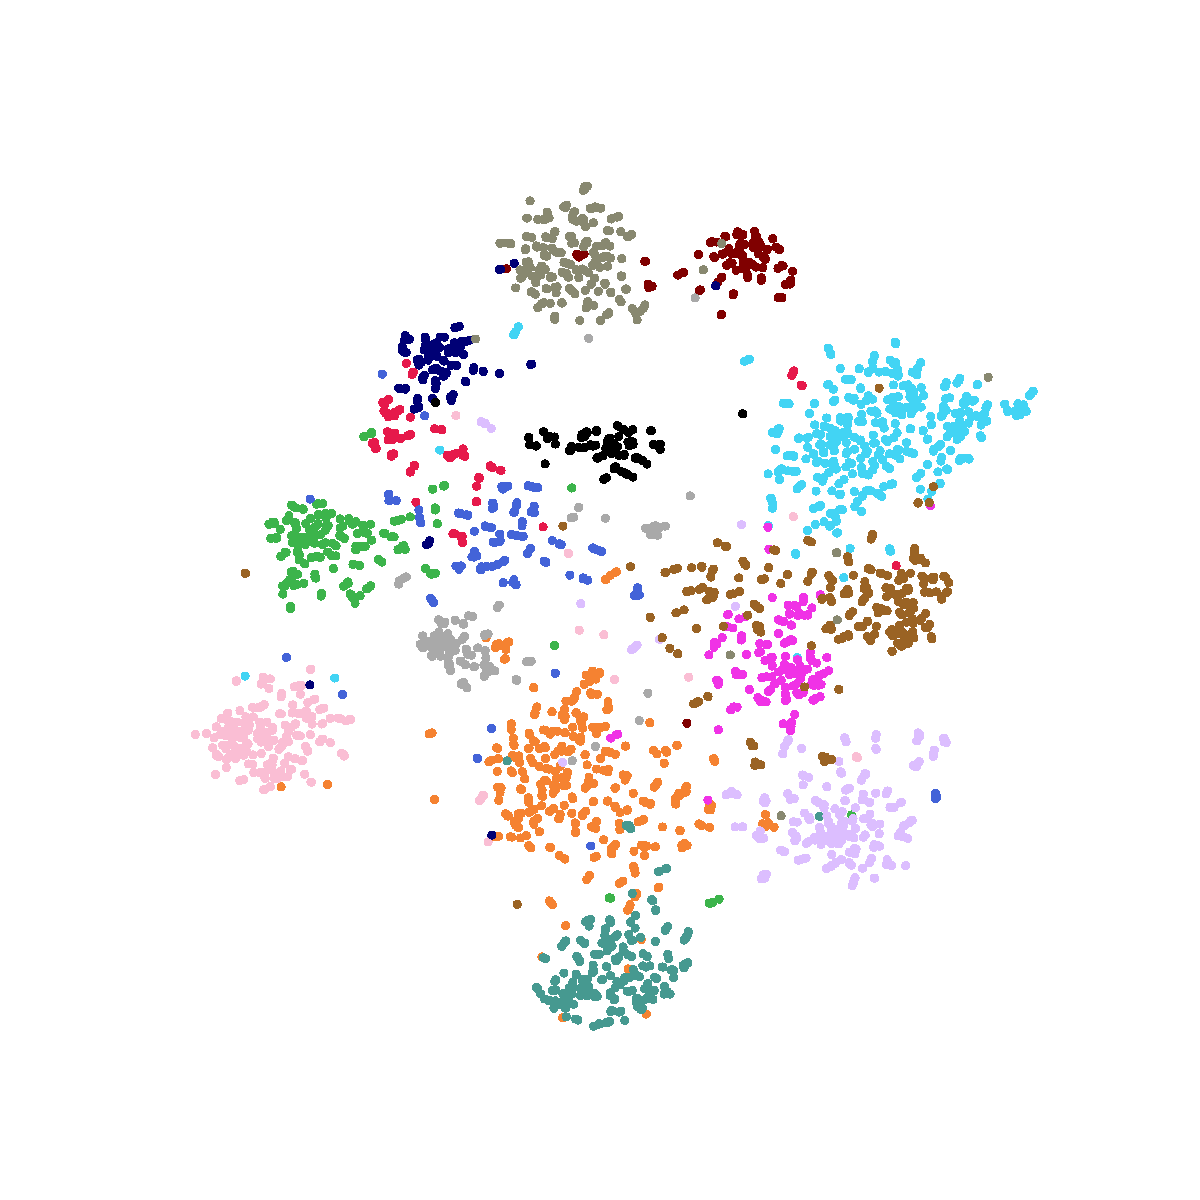
\includegraphics[width=0.5\linewidth]{fig/tsne/point_mae1.pdf}
        \caption*{\textbf{\#TP}:22.1M \textbf{\#OA}:80.25}
        \caption{1}
        \label{fig:sub1}
    \end{subfigure}
    \hfill
    \begin{subfigure}{0.24\textwidth}
        \centering
        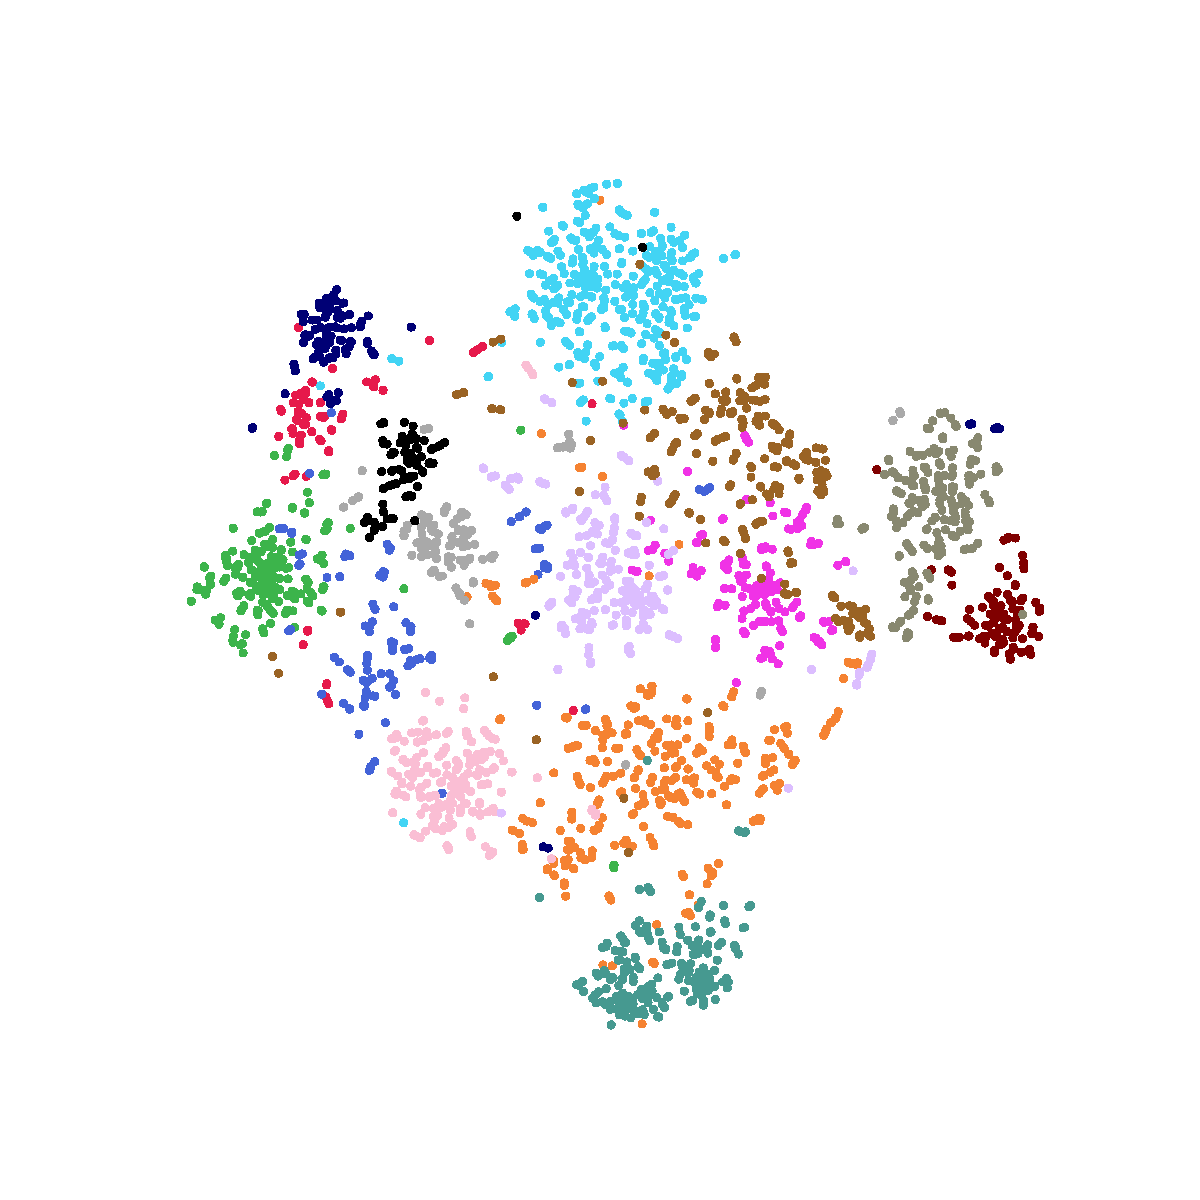
\includegraphics[width=0.5\linewidth]{fig/tsne/idpt1.pdf}
        \caption*{\textbf{\#TP}:22.1M \textbf{\#OA}:80.25}
        \caption{2}
        \label{fig:sub2}
    \end{subfigure}
    \hfill
    \begin{subfigure}{0.24\textwidth}
        \centering
        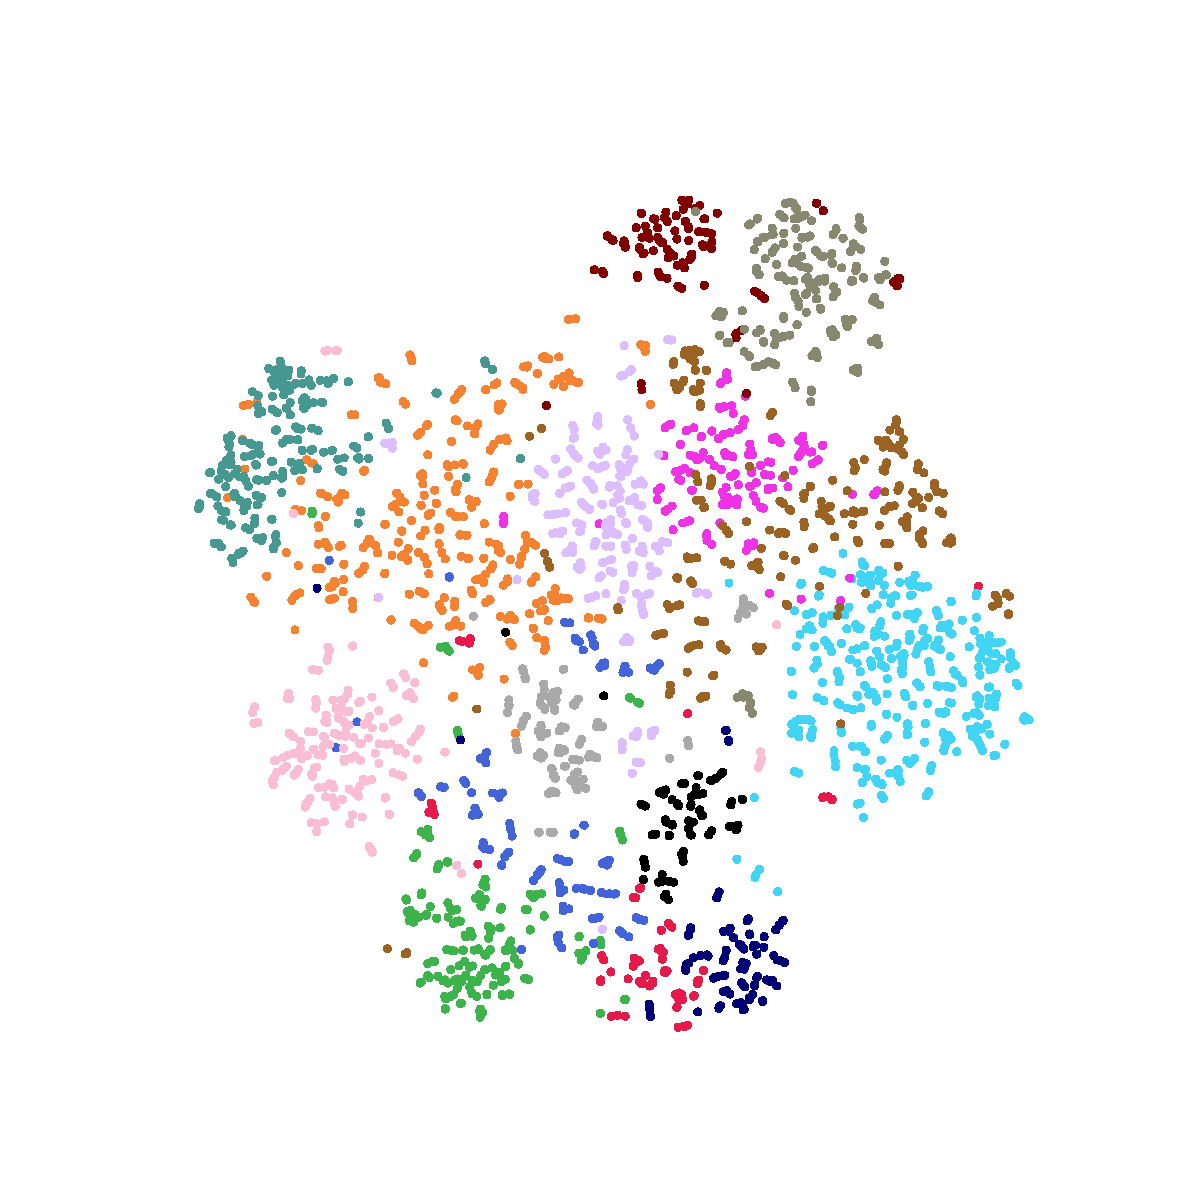
\includegraphics[width=0.5\linewidth]{fig/tsne/dapt1.pdf}
        \caption*{\textbf{\#TP}:22.1M \textbf{\#OA}:80.25}
        \caption{3}
        \label{fig:sub3}
    \end{subfigure}
    \hfill
    \begin{subfigure}{0.24\textwidth}
        \centering
        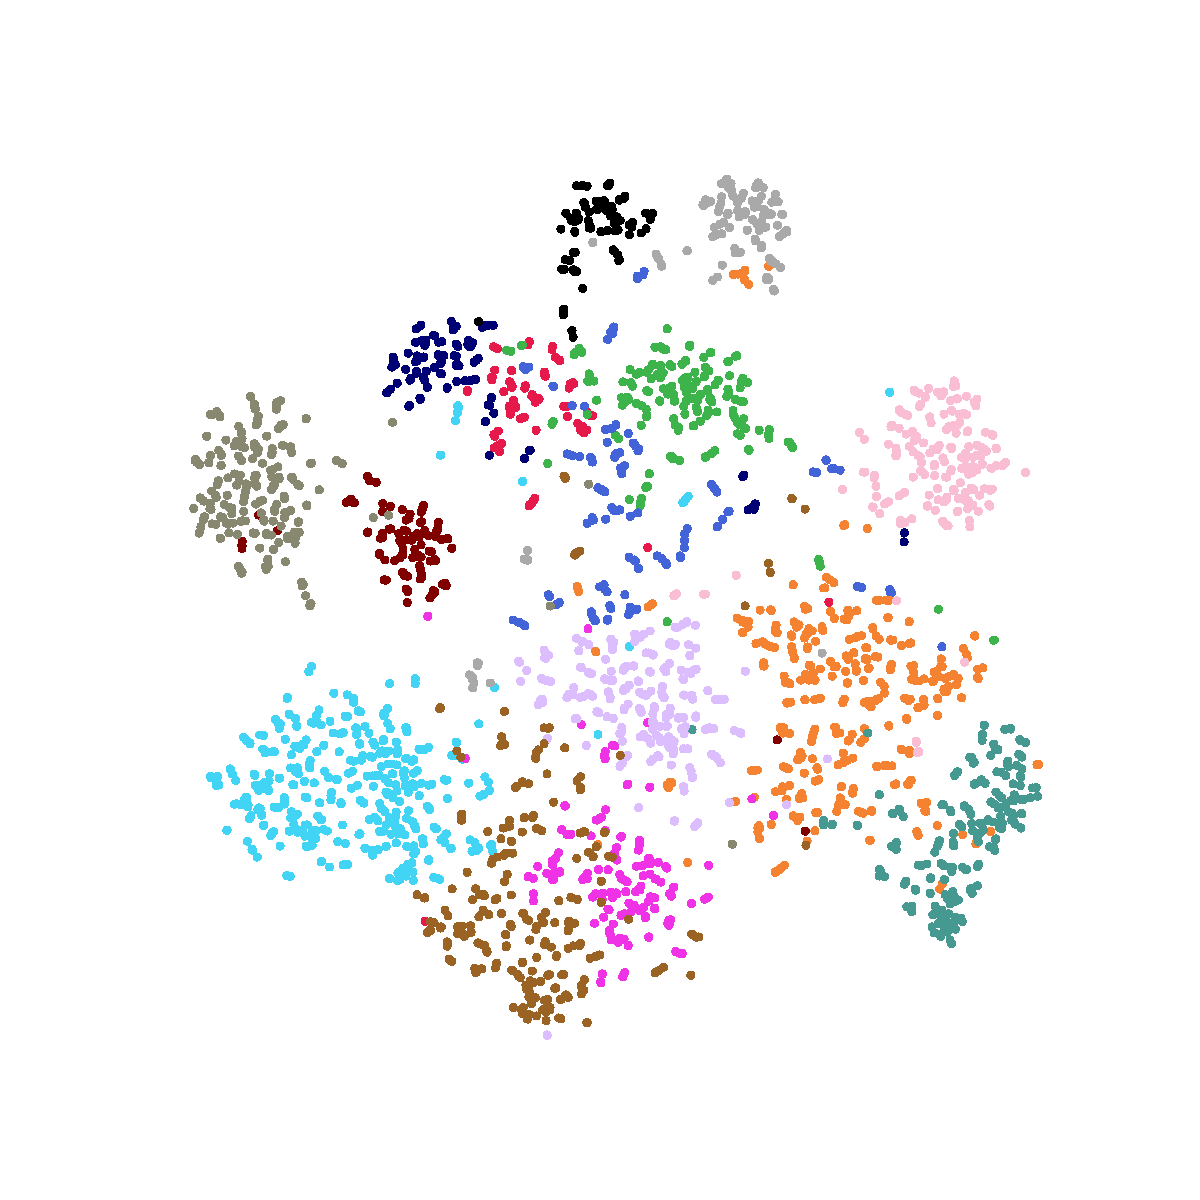
\includegraphics[width=0.5\linewidth]{fig/tsne/point_ladder1.pdf}
        \caption*{\textbf{\#TP}:22.1M \textbf{\#OA}:80.25}
        \caption{4}
        \label{fig:sub4}
    \end{subfigure}
    \caption{overall}
    \label{fig:whole}
\end{figure*}